\documentclass{article}
\usepackage{amssymb}
\usepackage{amsmath}
\usepackage{graphicx}

\begin{document}

\title{True Optics in 3D Rendering}
\author{Christian Oeien}
\date{August 19, 2016}
\maketitle

\begin{abstract}
A 3D renderer of basic geometric shapes of variable optics is presented.
The implementation created permits union and
intersection of spheres, planes, cylinders and cones
(and their spatial inverses)
each of parameterized reflection, refraction,
absorption and pass-through on semi-transparency.
Some optical phenomena are not accounted for by
the written program and this is discussed.
\end{abstract}

\section{Introduction}

The presented renderer is a ray-tracer, as described by \cite{raytrace}.
An alternative approach for rendering 3D is to project
each composed surface onto a raster.
Surfaces farther from the observer are overlayed by ones closer.
This projection technique is used for real-time rendering of moving 3D,
because ray-tracing requires much more calculation.
When creating a projection renderer two
problems arises immediately.  The surfaces may intersect, and even
tho they do not intersect a na{\"i}ve test for which surface to render first will fail
in many cases.  It is shown in \cite{linehide}
that the problems we encounter are not trivial.
And after these complex problems are solved, the result is still not
realistic.  The surfaces must somehow be shaded according to lighting
or reflexion.  This would be performed for the visible parts of the surfaces.
Also, for the realistic rendering of combined surfaces, there would be need for
some shading when applying the colors, as described in \cite{phongshade}.

For optical realism the ray-tracer technique is chosen.
This method arrives at realistic results
by itself, and with much simpler algorithms.
It must be noted that the CPU time
a program will need is bigger than for the projection technique for a picture
of comparable quality because of all the iteration and recursion done in ray-tracing.
In the technique of ray-tracing one seeks to calculate the color of each resulting pixel
in turn, by tracing the origin of the incoming light-ray from the corresponding direction.
Projection simulates the effects of light while
ray-tracing models each light-ray itself, on its journey from its
various sources.  The amount of information collected is limited because we
may on each combination perform filtering or addition of three components
of the simulated light.
If our visual ability was different, say
detecting all frequencies present like our auditory sense does, this
approach would not give a satisfying result.

Physically correct prism effect cannot be modeled with a
finite set of traced rays.  An attempt would be to implement the
ray-casting technique from the light-spot sources, which could
be limited to one traced ray per source at each absorbing surface.
But light dispersion shall also apply to the source light from other
objects, which would still require trace from infinite directions.
The presented ray-tracer ignores this problem by considering only a single
light-ray from any explicit light-source to an objects surface.

\section{Material and Methods}

The core engine is written in C
and the input-processing and
initial composition of the runtime scene of geometrical data
for all objects in C++.

The PC architecture is an Intel CPU with
\texttt{mmxext} and \texttt{sse4a} found in
\texttt{/proc/cpuinfo} running a Linux kernel.

\begin{figure}
  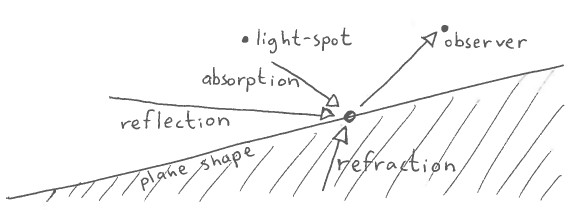
\includegraphics[width=\linewidth]{ray.jpeg}
  \caption{Tracer recursion}
  \label{fig:ray}
\end{figure}

\section{Results}

The source code is found at
\texttt{HTTP://github.com/biotty/rmg/graphics/ray}.
A separate software library for color manipulation was
factored out, and is found under
\texttt{graphics/rgb}.

For each pixel to generate, the program geometrically follows
the corresponding direction to the viewer.
The intersection of this ray with each object in the composed 3D scene
is calculated.
The closest point of intersection to the viewer is then
considered for reflexion, refraction and absorption at the hit surface.
Functions are called to find colors of incoming light that will
arrive in the direction of the viewer, at this point on the surface.
The normal vector (direction out of the 3D object) is also needed for
these calculations, where we recurse the procedure described, as if
we were a viewer at this point for light receiving reflection,
refraction and absorption per light point-source.  There is of-course
no recursion for refraction on an opaque object.  Absorption from
each spot light source is calculated.  When
no object is hit when tracing an incoming source light-ray for color,
we use the direction to calculate the color by one selected function
in \texttt{sky.c}.  Therefore the spot light sources
are not required to render color of a composed scene of objects.
Please see fig. \ref{fig:ray}.

While recursing through functions of optics and geometry
we operate a set of bits,
one per scene object, telling whether the view-location of our
currently traced ray is inside of that scene object.
Note that a traced ray may happen to start inside
of an opaque scene object,
because a transparent object may spatially overlap it
and its optics be in force at that location in space.

A basic geometric object must provide two functions
to our simulation.
For a given ray it calculates the distances to the
two intersections through it.  Then given a point
in space it gives a direction which will be the normal on its
surface.  Note that the fixation of maximum two intersections
means we cannot model a torus:
For a practical illustration, observe that four surfaces
of a donut touches your knifes blade if you cut it fairly.
In general we do not permit any concave (or saddle) surface.

The intersection is the only scene object that is composed
of other objects.  The intersection of shapes is the space
that is such that a point is included in all of those shapes.
Since the basic objects have no concave surfaces,
an intersection of them does not either.  A proof of this
is trivial, when using the mentioned observation of maximum
one segment (two intersections) of any line through such
an object:  An intersection of two segments can lead to no
more than one segment.
Please see fig. \ref{fig:inter}.

\begin{figure}
  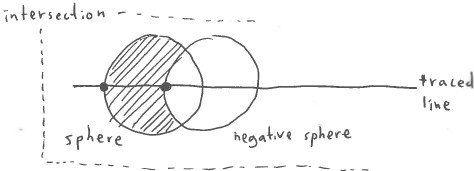
\includegraphics[width=\linewidth]{inter.jpeg}
  \caption{Set-intersection of shapes}
  \label{fig:inter}
\end{figure}

Negatives of the basic shapes except plane are supported
(negative planes would still allow for only planes).
A negation of a shape is modeled by considering that it
has the same enter-intersection and exit-intersection
with a ray, but the roles of enter and exit are swapped.

The calculations of intersections are complex but as
scene objects they have the same programatic interface,
and are traversed isomorphically to any scene object by
the core ray-tracer engine.  On the other hand, the support
for overlapping scene objects adds complexity to the
top-level ray-tracer algorithm itself.
A sequential order of scene objects is used to decide
precedence when traversing the geometrical boundary of
a scene object.  If inside of a scene object of higher
precedence than the traversed surfaces object, the ray
shall be traced as if the surface was not optically hit.
We need to know which scene objects we are geometrically
but not optically inside of.  Please see fig. \ref{fig:combi}.
This is accomplished with a stack data-structure
where we push or pop respectively when entering or exiting
an object through its surface with no optical presence.

\begin{figure}
  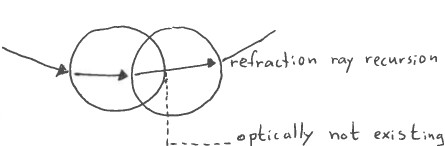
\includegraphics[width=\linewidth]{combi.jpeg}
  \caption{Overlap of scene objects}
  \label{fig:combi}
\end{figure}

The program takes a minimalistic syntax ASCII-encoded input,
and a Python module that feeds this to the ray-tracer
based on the equivalent composition using Python objects,
is provided.  This module also arranges for time-parametric
compositions so that sequences of images are generated,
to form motion-picture.

On my architecture I observed no difference in CPU time for
the three types of floating point.  The precision of the
calculations for a normal scene do not benefit from
the bigger types.  The data structures holding the geometrical
objects in the 3D scene uses the smallest type for spatial
coordinates and a compressed form of colors.

\section{Discussion}

The code that leverage C 11 and does not compile in C 99
is mostly found in for-loop constructs and idioms trivially
rewritten for C 99 if needed.  With C 11 a cast between
two \verb|struct| pointers where first member type is identical,
has defined behaviour by the language.
This is relevant for the scene object arguments, and we
need C 11 for us to be safe, even if the
practice of such casting was common in pre-2011 conformant
compilers.  Another type-problem is the \verb|struct|s for
direction and for point.  Casting between these types is
possible (the value itself, not a pointer)
because the compositions are identical.  However, it is not guaranteed
to result in a no-op runtime.  Also, use of different types
would let the compiler stop us from using the wrong type.
The source code arranges for the type-safe alternative of
using two different \verb|struct|s, by the alteration of one
preprocessor \verb|#define|.
The type of floating point used generally in the program is
also tunable.  This is done with \verb|typedef|.

In C we use \verb|void *| for holding the generic object data.
This could benefit from the type-system of C++.
The advantage of C is compilation-time.

I do not make use of an image-format software library
in my program, but merely feed raw color values and
facilitate for feeding this to a picture encoder, like the
available \texttt{pnmtojpeg} and use of \texttt{avconv}
on a typical Linux-based operating system.

The limitation on permittable shapes was arbitrary and because
I started with the simplest shapes without considering
other possibilities.  I had already implemented the
intersection algorithm when I got aware that there are
basic geometrical shapes that do not fit, and that my
algorithms had this constraint on intersection-pair.
The intersection algorithm was already complex,
and there was much work involved to make the floating-points
comparisons and the recursive splitting of the sections
in order to find the remaining intersection of all
component objects.  Adding to this complexity would
further increase CPU time spent on the tracing,
as the part spent in this code already showed to be
significant.

It must be noted that the physical phenomenon of
optical refraction is frequency-dependent,
and this is not modeled by the created ray-tracer.
This means that prism-like effects will not occur when
tracing through a transparent object.  If we were to model
this, it would not suffice to trace from only one direction
of refraction.  And any finite number of directions we chose
to trace would yield optically incorrect results.

The function that traces for absorption iterates over all
light-sources specified in the scene.  If the line between
the surface-point and a light-spot does anywhere hit a
surface of any scene object
then no color is applied from this light-source.
This means that total shadow is cast even from
a transparent object, and this is not physically correct.
The problem is of finding what path a light-ray would take
through transparent objects to reach a given point.
A solution to this problem would be computationally intensive,
and when implemented we would still not obtain the
prism effect due to the other problem as described previously.
I chose to focus on implementing the optically
correct simulations and to conserve simplicity.

\bibliographystyle{plain}
\bibliography{optic}

\end{document}
